This section first describes the prototypes we have developed as proof-of-concept to illustrate feasibility (Section~\ref{sec:prototypes}).
Then it describes our plan for the implementation of SAInT (Section~\ref{sec:design:implementation}).

\subsection{Prototypes Developed}
\label{sec:prototypes}
We have begun prototyping the feasibility of some of the key requirements. 
The following subsections briefly summarize these prototypes and how that work leads to the plan for SAInT.

\subsubsection{Feasibility of Data Interchange (Requirements 7, 8, and 9)}
Undergraduate students working in the UA REU program managed by PI Carver (CCF-1156563) investigated what would be involved in supporting data interchange among SLR phases and tools.
The student focused on the searching and selection process, because of its importance.
The students were able to programmatically clean and populate the results of a search in various digital libraries (ACM, IEEE, Engineering Village) into a database.
This prototype illustrated the feasibility of manipulating and standardizing the results from different digital libraries so they can be stored in a local database. 
The lessons learned during this exercise will be important for construction of the API of SAInT to ensure easy interaction with other tools.

\subsubsection{Feasibility of Programmatically Accessing Literature Databases - (Requirement 1 and 2)}
The search and selection steps in the SLR process are complicated by the functionality currently provided by the major literature databases (i.e. ACM, IEEE and Springer). 
It was also one of the most important tooling needs indicated by our survey and workshops.
We asked the REU students to design and build a prototype to overcome some of the barriers in the search phase. 
The search process consists of multiple sub-problems (i.e. building the search query, searching the databases, downloading results, parsing the results into a local database, and eliminating duplicates).
In the course of their research, the students discovered that the public APIs provided by the major digital libraries (i.e. IEEE, ACM, Springer, and Engineering Village) did not adequately support automated searching, reference downloading, or reference manipulation.

Subsequently, we pursued the automated searching problem in more detail.
We initiated discussions with two of the major digital library providers: IEEE and ACM. 
Upon hearing of the goals of our proposed work, both organizations responded favorably to our requests for access to their APIs.
Using those APIs, we began work on a tool to assist in automated searching. 
Even though the APIs were early in their development, we were able to tweak them to build a prototype for an automated searching tool. 
The tool currently assists with searching the ACM and IEEE digital libraries and automatically downloading the results.

\subsection{Design and Implementation of SAInT}
\label{sec:design:implementation}

SAInT enables a coordinated approach to facilitate the authoring of SLRs, covering each SLR phases from planning to dissemination of the results. 
At a high level of abstraction, SAInT will consist of functional tool features to:
\begin{enumerate}
	\item support SLR Authors in each phase,
	\item support cross-phase coordination and revised planning, and 
	\item maintain queries, protocols, article links, and meta-data.
\end{enumerate}

Figure~\ref{fig-architecture} depicts how the capabilities of SAInT map onto the SLR process.   
Vertically, each phase of the SLR has its corresponding support features.
Because SAInT is based on an open architecture, the support features may be provided by existing tools, as a plug-ins, and/or by tools that we develop as part of this project. 
Integral to SAInT is the \textit{Centralized Storage} repository that provides persistence to data, meta-data, statistics, and literature.

\begin{figure}
	\centering
	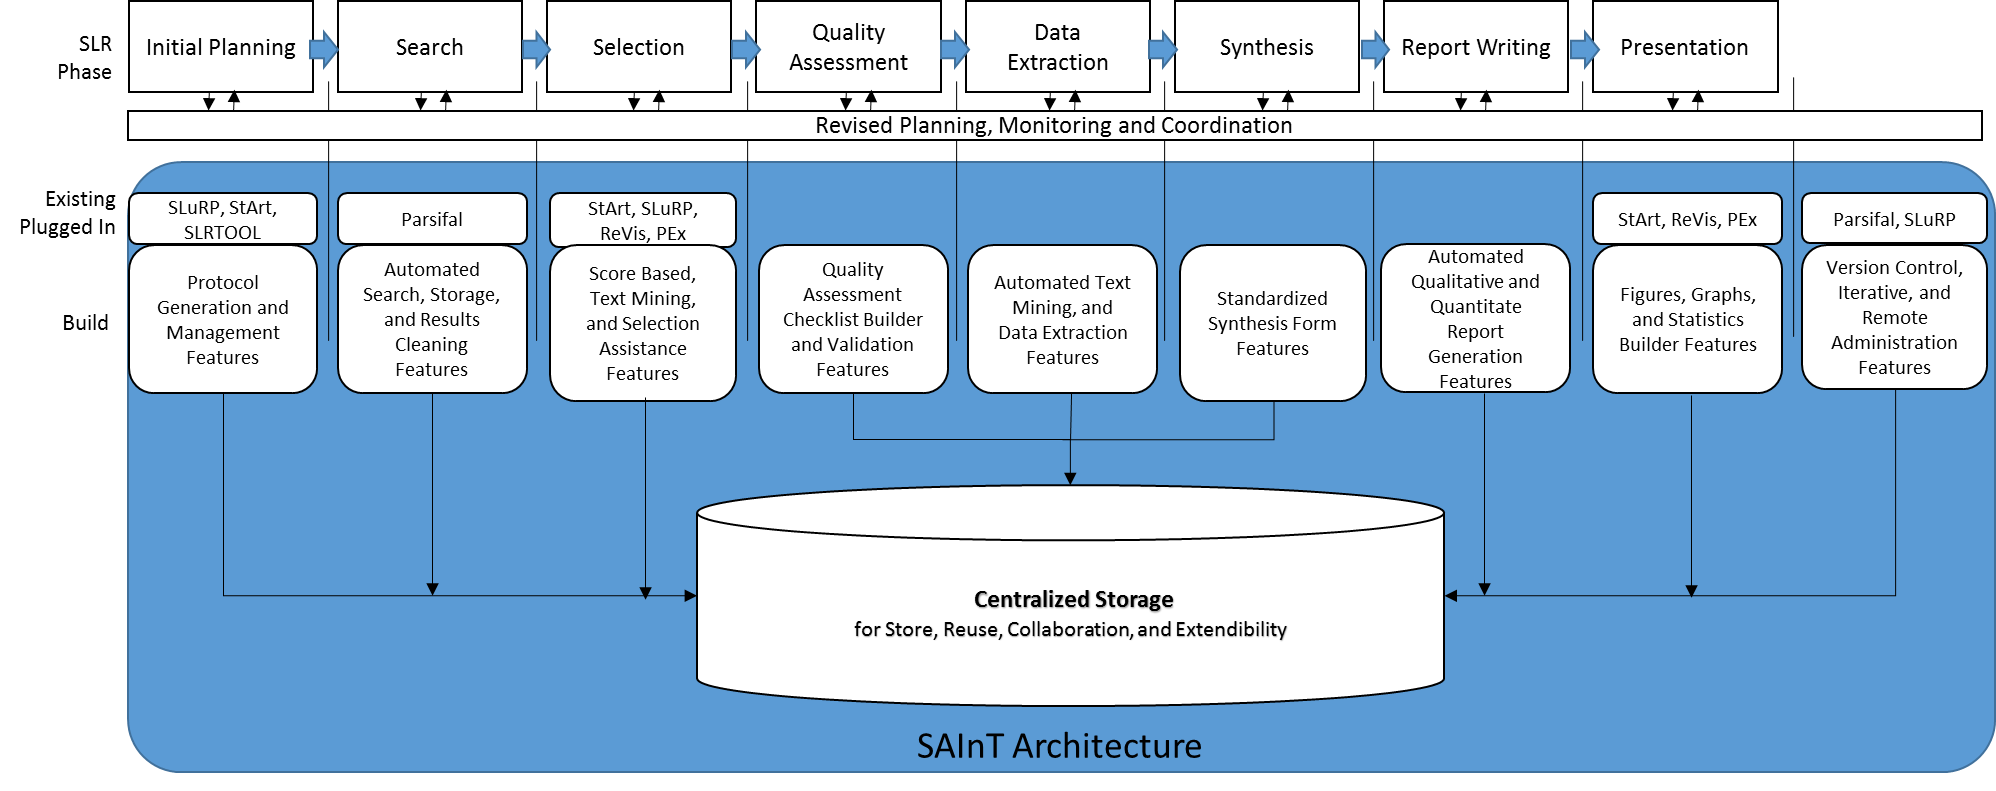
\includegraphics[width=\textwidth]{Architecture}
	\caption{High-Level Architecture}
	\label{fig-architecture}
\end{figure}

SAInT will implement the following functionality to support the four guiding principles enumerated in Section~\ref{sec:intro}.
\begin{enumerate}
	\item Automation of tasks in each of the SLR phases, thus reducing manual labor and as will support iteration.  
	\item Facilitation of collaboration of multiple researchers working on the same and different phases through data exchange both within and between phases. 
	\item Support of reuse and evolution through the centralized data store that is available to tools in each of the SLR authoring phases.  
	\item Providing an open ecosystem to enable the use of existing and future tools developed by other organizations. The architecture has APIs and embedded data exchange features. Thus, tools that provide partial support for the SLR authoring process (see Table~\ref{table-tools}) can be plugged into SAInT. 
\end{enumerate}

Based on this functionality, the SLR process described in Figure~\ref{figure-SLR-Process}, and the requirements from Section~\ref{sec:results:workshops}, Table~\ref{table-features} provides a list of some of the features we will build into SAInT.  

%To illustrate the next level of detail we have developed for each of these features during our planning grant, the Selection Phase inclusion/exclusion criteria for articles feature will include the ability to assess the technical measures (e.g., recall and precision) for achieving acceptable screening (i.e., culling) of articles.   
%These measures provide a means for researchers to ensure the completeness and unbiased nature of the dataset for the review.

\begin{table}
	\centering
	\caption{Sample Features provided by SAInT}
	\resizebox{15cm}{!}{
	\begin{tabular}{|m{3cm}|m{12cm}|}
		\hline
		\textbf{SLR Phase} & \textbf{Sample High-Level Features (Requirement Number in parenthesis)*} \\
		\hline
		Initial \newline Planning & Generate Project ID, SLR Protocol definition, Facilitate topic refinement, Establish team membership, Designate roles, Initialization of repository, \textbf{Import of validated protocols (R10)}, and a \textbf{Discussion forum (R4)} \\
		\hline
		Search & \textbf{Standardized query language translate to specific archives (R10)}, Storage
		of queries and their resulting data sets, Support for synonym expansion and
		stemming, \textbf{Snowballing support, Deduplication (R1)}, \textbf{Data import/export
		facilities (R8)}, and \textbf{Metadata/Statistics (R5)} \\
		\hline
		Selection & Support for inclusion/exclusion criteria for articles, \textbf{Automated inclusion/
		exclusion of studies (R1)}, \textbf{Text Minded Extractions (R10)}, \textbf{Data import/
		export facilities (R8)}, and \textbf{Metadata/Statistics (R5)} \\
		\hline
		Quality \newline Assurance &
		Adherence to protocol, Assessment of Metadata and statistics, \textbf{Standardized
		checklists for data quality (R2)}, Traceability, and a Forum for discussion \\
		\hline
		Data \newline Extraction &
		Text Mining, Assisted Coding, Piloting, \textbf{Data Interchange and APIs (R8 \&
		R9)}, Translation to common data format, and Clipboards \\
		\hline
		Synthesis & \textbf{Data Interchange (R8)}, \textbf{APIs to advanced statistical tools (R9 \& R10)}, Conflict resolution, and a Forum for discussion \\
		\hline
		Report \newline	Writing &
		\textbf{Data Interchange (R8)}, APIs to advanced publishing tools, and a \textbf{Forum
		for discussion (R9 \& R10)} \\
		\hline
		Presentation & \textbf{Data Interchange (R8)}, \textbf{APIs to advanced visual analytic tools (R9 \& R10)} \\
		\hline
		Revised \newline Planning, \newline	Monitoring \& \newline	Coordination &
		Forum for discussion, Resource planning, \textbf{Version control (R3)}, \textbf{Change
		management for revised planning (R6)}, Documentation, Generate a new
		Project ID, \textbf{Revise SLR Protocol (R7)}, change team membership and role,
		and Curation of repository\\
		\hline
	\end{tabular}
}
\newline
\small{*Bold features indicate the Top 10 high-level requirements listed in Section 4.3}
	\label{table-features}
\end{table}

